\section{Constitution du modèle}

Notre problèmatique est centrée autour de la constitution d'un système d'authentification en l'absence de données d'imposteurs.

À l'aide de la base de données du GREYC, nous avons pu tracer sur la figure~\ref{3d}, sur trois dimensions, le positionnement des mesures pour deux utilisateurs distincts. On peut noter que même dans un nombre faible de dimensions, il semble possible de séparer les mesures en deux groupes distincts représentant chacun un utilisateur. S'il est possible de grouper les données de deux utilisateurs distincts, il est donc possible de définir une frontière de décision qui permet de définir si une nouvelle mesure fait partie ou non d'un groupe donné. On appelle ceci un algorithme de \textit{novelty detection}.

\begin{figure}[b]
    \centering
    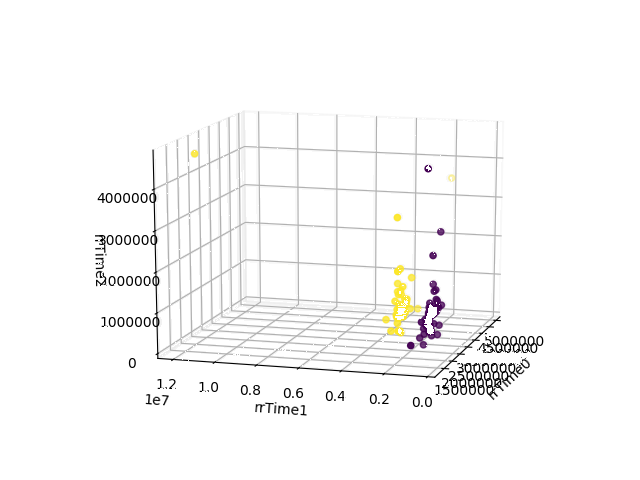
\includegraphics[width=\linewidth]{res/3d.png}
    \caption{Affichage des mesures de l'utilisateur 1 et de l'utilisateur 2 de la base GREYC en fonction des valeurs \textit{rrTime0}, \textit{rrTime1}, \textit{rrTime2}}
    \label{3d}
\end{figure}

Le principal algorithme de \textit{novelty detection} présent dans la librairie \textit{scikit-learn} est l'algorithme de \textit{One-Class SVM}.

Notre travail tente de produire un modèle biométrique basé sur cet algorithme en suivant la méthodologie résumée dans la figure~\ref{ocsvm}, qui récapitule le processus de traitement des données, de constitution du modèle, et d'évaluation de ce même modèle.

\subsection{Pré-traitement des données}

Les données nécessitent d'abord un pré-traitement. Selon la publication \textit{A Practical Guide to Support Vector Classification \cite{svmpractical}}, les données doivent être mises à l'échelle $[0, 1]$ ou $[-1, 1]$. Notre choix s'est porté sur l'échelle $[0, 1]$, qui mettait en évidence de meilleurs résultats lors de l'évaluation des tests préliminaires.

\label{modele}
\subsection{Entraînement du modèle}

L'entraînement du modèle se fait uniquement sur les données utilisateur, c'est-à-dire des données uniquement \textbf{positives}, le jeu de données ne comportant pas d'exemple de données d'imposteurs. Comme pour nombre de modèles d'apprentissage machine, nous divisons les données en deux lots :

\begin{itemize}
    \item Un lot de données d'entraînement
    \item Un lot de données d'évaluation
\end{itemize}

D'une manière génèrale, il est recommandé d'assigner $4/5$ des données à l'entraînement et $1/5$ des données à l'évaluation. Cette répartition est faite automatiquement lors de la recherche des meilleurs paramètres à l'aide d'un algorithme de \textit{k-fold} : l'entraînement d'un modèle est fait $k$ fois, avec $k$ séparation des données différentes, de manière à trouver les meilleurs coefficients.

Le lot de données d'évaluation est utilisée pour optimiser les paramètres du modèles. Habituellement, cette optimisation se fait à l'aide d'une \textit{recherche par grille de paramètres}, en recherchant les paramètres qui permettent d'obtenir la meilleure précision. Or, dans le cas d'un modèle entraîné sans données d'imposteurs, il n'est pas possible d'obtenir une évaluation de la précision fiable. Il faut donc utiliser une autre mesure pour l'évaluation du modèle : le \textit{rappel}.

Le rappel est "la proportion des items pertinents proposés parmi l'ensemble des items pertinents". Autrement dit, il s'agit de l'ensemble des données détectées comme étant des données utilisateurs sur le nombre effectifs de données utilisateurs. Cette définition n'implique pas la présence de données imposteurs et convient donc à l'évaluation de notre modèle pour la recherche des meilleurs paramètres. Nous chercherons alors à obtenir un rappel qui tend vers 1.

\subsection{Évaluation du modèle}

Une fois le modèle entraîné, nous pouvons l'évaluer avec des données d'imposteurs. Il faut noter ici que cette phase d'évaluation ne sera pas possible lors de l'implémentation d'un logiciel d'authentification par la dynamique de frappe au clavier, en l'absence de données d'imposteurs. Nous l'utilisons ici pour évaluer notre méthode d'entraînement du modèle.

Pour l'évaluation, nous utilisons toutes les données à notre disposition. Les données utilisateurs seront d'abords divisées en deux lots (un d'entraînement et un d'évaluation). Les données d'entraînement sont passées au module d'entraînement. Le modèle résultant est alors évalué à l'aide des données d'évaluation. On s'intéresse ici au \textit{f-score}, qui est une métrique équilibrant les notions de \textbf{rappel} et de \textbf{précision} pour produire un score significatif.

\begin{figure}[]
    \centering
    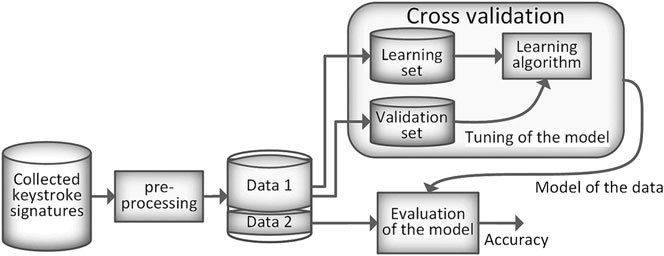
\includegraphics[width=\linewidth]{res/ocsvm.png}
    \caption{Chaîne d'entraînement et d'évaluation d'une One-Class SVM selon Thierry Eude et Chuan Chang\cite{doi:10.1111/coin.12122}}
    \label{ocsvm}
\end{figure}
